Question:\\
\emph{
    Design a DW that should be used at Census Bureaus. Logical design only.\\ Focus on only
one fact + five dimensions.\\ 5 attributes per table are required.\\ The point should include
measures. Relationships should be shown.
}\\\\
\emph{[00:10:33] then fourth question is about design question so this is where you design a data warehouse but then do i need to design a fully
fledged end to end the data warehouse for a census office no that's not required so here it's a logical
design focus on one factor plus five dimensions so this is like a small uniscope data warehouse five
attributes per table are required and the points should also include uh the measures uh in the fact
five attributes on the dimension and the measures on the facts and then you need also to show the
relationship like i have explained um in this week's lecture about the one to many relationships
yeah which now some students usually ask yeah what is it about yeah that that is where you have freedom
to decide so um if i go back here just to give you some more explanation on this question if i go here
so this is of course that's not a data warehouse model these are the areas about which the census offices
collect and maintain data and offer insights uh to those interested yeah so for example you might
say i will do my star schema data warehouse about the population so you need to have
fact and five dimensions about population another student would come and say i will do it about fishery and
then third i will do it about trade and i will do it about housing which one do you choose this is up to you
so i leave that in your hands uh subject to your interest uh yeah you decide uh yeah on question number four
four}\\\\
What to do here?
\begin{enumerate}
    \item decide 1 fact and 5 dimensions to use
    \item make a dimension diagram
    \item include relationships
    \item decide attributes (at least 5 per table)
  \end{enumerate}

\newpage Answers to Question 4:
\section{Logical design of a data warehouse for Census Bureaus}
We have designed a limited dimensional model that could be implemented by a Census Bureau. The model is classified as star schema as it has only fact table which is connected to a number of denormalized dimension tables (Coursebook, 32.4). The theme chosen for this star schema was residence permits in Sweden, which constitutes a part of migration and which among Census Bureaus belongs to the subject area “Population”. Depending on the scope and perspective, residence permits potentially also connects to “Living conditions” and “Housing”. The motivation of us to design a DW about residence permits is mainly to obtain a statistical tool that creates insights about persons who have been granted residence permits in Sweden. As to first gain a better understanding of common features among the target group, and then to help local, regional and national decision makers in Sweden to improve the overall lives of persons with residence permits. 
\\\\
The star schema that the group created consists of the fact table ResidencePermits, whose primary key is a composite key consisting of five foreign keys stemming from each dimension table. The fact table contains three fact attributes or facts, which are: permanentResPermits, temporaryResPermits and totalResPermits. As the table name and fact attributes suggest, they refer to the quantitative number of residence permits granted to individuals in a certain country, in this example in Sweden. Here the residence permits have been divided into two additive types, permanent and temporary. Also, total permits has been included, which is registered separately but which should equal the sum of the former two types. 
\\\\
The fact table has been accompanied by five dimension tables. Each one of these contains one surrogate type of primary key together with five attributes relating to the dimension in question. The measures of the attributes vary within and across dimension tables, but most of them are qualitative. All five dimensions Time, Domicile, Background, Socioeconomics and Living – including their attributes – have relationships with ResidencePermits as the fact being analysed. It is worth noting that the individual facts in the fact table are independent from all other attributes in the dimension tables, except for the two attributes residencePermitCat and residencePermitDate, which are implicitly interrelated with each of the three facts (permanentResPermits, temporaryResPermits and totalResPermits). 
\newpage
\subsection{Fact table and dimension tables (star schema)}
\begin{figure}[h] % "h" means "here"
  \centering
  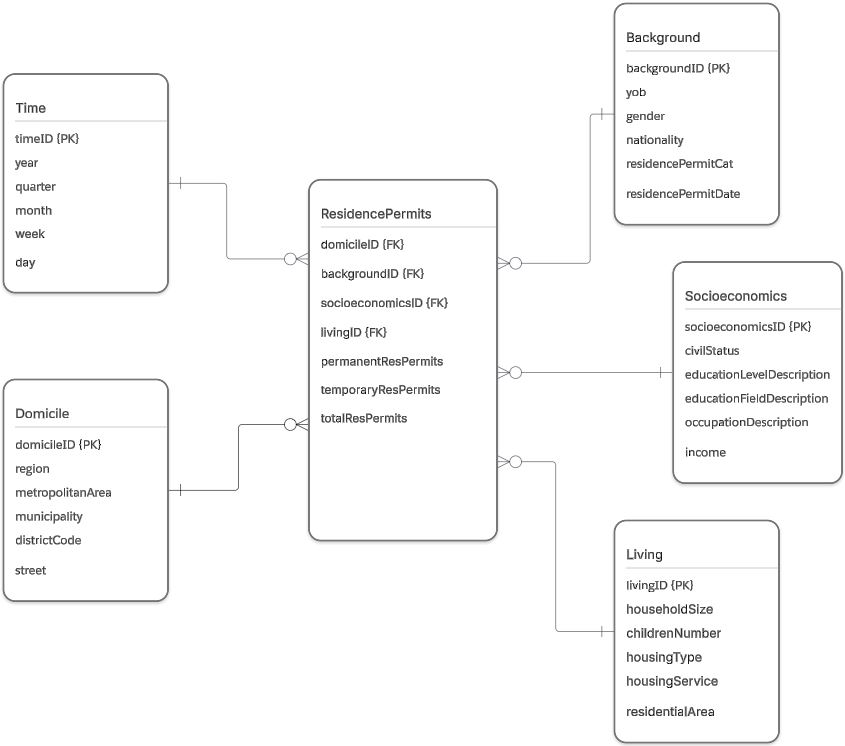
\includegraphics[width=1.0\textwidth]{Figures/Q4_StarSchema.jpg}
  \label{fig:my_image}
\end{figure}
\newpage
\subsection{Attribute descriptions for logical design}
% ResidencePermits (Fact table)
\begin{table}[htbp]
  \centering
  \caption{ResidencePermits (Fact table)}
  \begin{tabular}{|l|l|l|}
    \hline
    \textbf{Attribute} & \textbf{Domain} & \textbf{Data type} \\
    \hline
    timeID & Foreign Key & INT \\
    \hline
    foreignID & Foreign Key & INT \\
    \hline
    domicileID & Foreign Key & INT \\
    \hline
    backgroundID & Foreign Key & INT \\
    \hline
    socioeconomicsID & Foreign Key & INT \\
    \hline
    livingID & Foreign Key & INT \\
    \hline
    permanentResPermits & Number of granted permanent resident permits & INT \\
    \hline
    temporaryResPermits & Number of granted temporary resident permits & INT \\
    \hline
    totalResPermits & Total number of granted resident permits & INT \\
    \hline
  \end{tabular}
\end{table}

% Time (Dimension table)
\begin{table}[htbp]
  \centering
  \caption{Time (Dimension table)}
  \begin{tabular}{|l|l|l|}
    \hline
    \textbf{Attribute} & \textbf{Domain} & \textbf{Data type} \\
    \hline
    timeID & Primary Key, auto increment & INT \\
    \hline
    year & Year & INT \\
    \hline
    quarter & Quarter of a year & SMALLINT(1-4) \\
    \hline
    month & Month & SMALLINT(1-12) \\
    \hline
    week & Week & SMALLINT(1-53) \\
    \hline
    day & Day & SMALLINT(1-31) \\
    \hline
  \end{tabular}
\end{table}

% Domicile (Dimension table)
\begin{table}[htbp]
  \centering
  \caption{Domicile (Dimension table)}
  \begin{tabular}{|l|l|l|}
    \hline
    \textbf{Attribute} & \textbf{Domain} & \textbf{Data type} \\
    \hline
    domicileID & Primary Key, auto increment & INT \\
    \hline
    region & Region & VARCHAR \\
    \hline
    metropolitanArea & Metropolitan area & VARCHAR \\
    \hline
    municipality & Municipality & VARCHAR \\
    \hline
    districtCode & District code & VARCHAR \\
    \hline
    street & Street & VARCHAR \\
    \hline
  \end{tabular}
\end{table}

% Background (Dimension table)
\begin{table}[htbp]
  \centering
  \caption{Background (Dimension table)}
  \begin{tabular}{|l|l|l|}
    \hline
    \textbf{Attribute} & \textbf{Domain} & \textbf{Data type} \\
    \hline
    backgroundID & Primary Key, auto increment & INT \\
    \hline
    yob & Year of birth & SMALLINT(4) \\
    \hline
    gender & Gender & CHAR(1) \\
    \hline
    nationality & Nationality & VARCHAR \\
    \hline
    residencePermitCat & Residence permit category (Family/Work/EU-EES/Asylum/...) & ENUM \\
    \hline
    residencePermitDate & Date of residence permit & DATE \\
    \hline
  \end{tabular}
\end{table}

% Socioeconomics (Dimension table)
\begin{table}[htbp]
  \centering
  \caption{Socioeconomics (Dimension table)}
  \begin{tabular}{|l|l|l|}
    \hline
    \textbf{Attribute} & \textbf{Domain} & \textbf{Data type} \\
    \hline
    socioeconomicsID & Primary Key, auto increment & INT \\
    \hline
    civilStatus & Civil status & VARCHAR \\
    \hline
    educationLevelDescription & Education level & VARCHAR \\
    \hline
    educationFieldDescription & Field of education & VARCHAR \\
    \hline
    occupationDescription & Occupation category & VARCHAR \\
    \hline
    income & Yearly gross income in 1000 Swedish Kr & DECIMAL \\
    \hline
  \end{tabular}
\end{table}

% Living (Dimension table)
\begin{table}[htbp]
  \centering
  \caption{Living (Dimension table)}
  \begin{tabular}{|l|l|l|}
    \hline
    \textbf{Attribute} & \textbf{Domain} & \textbf{Data type} \\
    \hline
    livingID & Primary Key, auto increment & INT \\
    \hline
    householdSize & Number of persons in the household & TINYINT \\
    \hline
    childrenNumber & Number of children in the household & TINYINT \\
    \hline
    housingType & Type of housing (building type \& ownership type) & VARCHAR \\
    \hline
    housingService & Housing service (service housing/ /facility/supervised camp/...) & VARCHAR \\
    \hline
    residentialArea & Residential area in square meters, m2 & DECIMAL \\
    \hline
  \end{tabular}
\end{table}